\chapter{Processo Unificato}
\label{chap:processo-unificato}
Il \textbf{processo unificato} (o \textbf{UP}, \textbf{Unified Process}) è un processo di sviluppo software \hyperref[process-model:iterativi]{iterativo} con le seguenti caratteristiche:
\paragraph{Incentrato sull'architettura} L'{architettura} del sistema viene definita dalle prime \hyperref[process-model:iterativi]{iterazioni}.
\paragraph{Basato sul rilascio incrementale} Concetto già spiegato nella sezione \hyperref[concept:rilascio-incrementale]{apposita}.
\paragraph{Incentrato sul rischio} Tutte le scelte, specialmente nelle fasi iniziali del processo, vengono prese prioritizzando la riduzione del {rischio}.
\paragraph{Guidato dai casi d'uso} I \hyperref[concept:casi-duso]{casi d'uso} sono usati per definire e specificare i requisiti.
\paragraph{Iterazioni time-boxed} Le iterazioni seguono precise scadenze entro le quali devono essere concluse. 

\section{Struttura dell'UP}
\label{concept:UP-structure}
Lo Unified Process è strutturato a \textbf{fasi}. Una fase comprende più iterazioni. In ogni fase sono prioritirizzate alcune attività rispetto ad altre. Alla fine di ogni iterazione viene generata una {baseline}, questa viene valutata secondo alcune precise condizioni che, se verificate, dichiarano conclusa la fase. La {baseline} che verifica queste condizioni viene detta \textbf{milestone}. Le fasi del Processo Unificato sono \textbf{quattro}: \hyperref[concept:avvio]{avvio}, \hyperref[concept:elaborazione]{elaborazione}, \hyperref[concept:costruzione]{costruzione} e \hyperref[concept:transizione]{transizione}.
\begin{figure}[h]
    \centering
    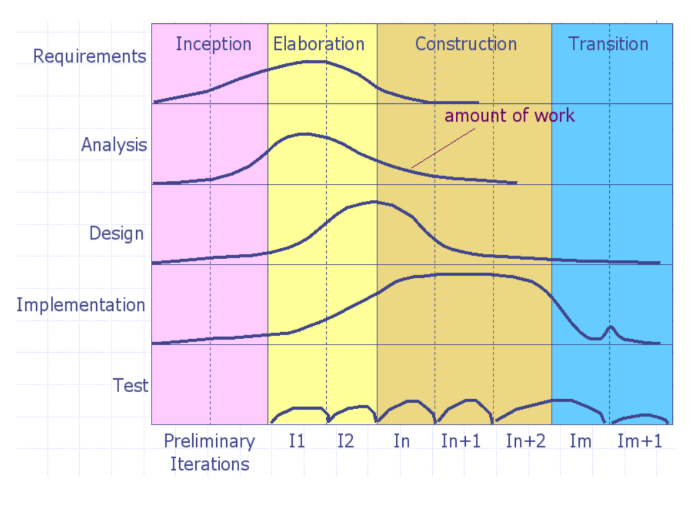
\includegraphics[width=0.75\linewidth]{IDSTEORIA//Immagini/ProcessoUnificato/UPStructure.png}
    \caption{Distribuzione delle varie attività nelle fasi dell'UP}
    \label{fig:UPStructure}
\end{figure}
\subsection{Avvio (o Inception)}
\label{concept:avvio}
\paragraph{Attività Principali} Identificazione degli {stakeholder}, raccolta dei requisiti ad alto livello, definizione di uno Use Case Diagram iniziale, stima dei costi, analisi di fattibilità, valutazione dei rischi, definizione di un piano di progetto.
\paragraph{Obiettivi} Definire ambito del sistema, identificare principali casi d'uso, valutare la fattibilità del progetto, stabilire un business case solido.
\paragraph{Milestone}
\begin{itemize}
    \item UC Diagram contenente 10-20\% dei Casi D'Uso ben definiti
    \item Go-no go: decisione se il progetto è fattibile e vale la pena continuare
    \item Business case
    \item Vision document
    \item Lista ed analisi dei rischi
\end{itemize}
\subsection{Elaborazione (o Elaboration)}
\label{concept:elaborazione}
\paragraph{Attività Principali} Sviluppo dell'architettura software, completamento di use case significativi, definizione dell'architettura del sistema, inizio della documentazione tecnica, valutazione di rischi tecnici tramite prototipi. ù
\paragraph{Obiettivi} Definire e validare architettura software, affinare i requisiti, ridurre i rischi più significativi, produrre un piano di progetto dettagliato per le fasi successive.
\paragraph{Milestone}
\begin{itemize}
    \item UC Diagram contenente 80-90\% dei Casi D'Uso ben definiti
    \item Architettura stabile ed \textbf{eseguibile}
    \item Piano di progetto revisionato
    \item Stima dei rischi revisionata
    \item Accordo finale tra le parti firmato
\end{itemize}
\subsection{Costruzione (o Construction)}
\label{concept:costruzione}
\paragraph{Attività Principali} Sviluppo iterativo del software completo, implementazione completa dei casi d'uso, scrittura, ottimizzazione, testing e documentazione del codice, gestione di eventuali cambiamenti nei requisiti, rivalutare i rischi.
\paragraph{Obiettivi} Completare l'identificazione, la descrizione e l'implementazione dei Casi D'Uso, mantenere l'integrità dell'architettura del sistema. 
\paragraph{Milestone}
\begin{itemize}
    \item Software stabile e di qualità sufficiente da essere rilasciato
    \item Verifica dei costi rispetto alla pianificazione iniziale
    \item Eventuali manuali o piani di distribuzione definiti nell'accordo tra le parti
\end{itemize}
\subsection{Transizione (o Transition)}
\label{concept:transizione}
\paragraph{Attività Principali} Testing lato utente, modifiche del design in caso siano emersi errori in fase di testing, supporto tecnico e documentazione, raccolta di feedback degli utenti, refactoring o ottimizzazione finale.
\paragraph{Obiettivi} Rilascio prodotto agli utenti finali, correzione errori, addestramento e supporto agli utenti per l'utilizzo del software.
\paragraph{Milestone}
\begin{itemize}
    \item Prodotto software ultimato e testato
    \item Uso attivo del prodotto
    \item Definizione delle strategie di supporto (es. manuale utente)
    \item Piano di Manutenzione
\end{itemize}

\section{Casi d'Uso}
\label{concept:casi-duso}
Un \textbf{Caso D'Uso} (o \textbf{CU} o \textbf{Use Case} o \textbf{UC}) è un insieme di scenari volti al descrivere un'interazione tipica tra un {attore} e il sistema per raggiungere un obiettivo specifico. I casi d'uso rappresentano le funzionalità osservabili dall'esterno e descrivono come il sistema risponde agli input degli attori (\textbf{passività del sistema rispetto all'attore}). Nel contesto del Processo Unificato, i Casi d'Uso sono il principale strumento per la definizione e specifica dei {requisiti} del sistema. 
\subsection{Come individuare gli attori?}
\label{individuazione-attori}
Il primo passo per l'individuazione e definizione dei casi d'uso e l'individuazione degli {attori} che andranno ad attivarli. Un \textbf{attore} rappresenta un ruolo che un'entità può assumere. E' importante notare che un'entità può assumere più ruoli e quindi impersonare più attori. L'individuazione degli attori avviene attraverso una serie di domande relative alle funzioni che il team si pone:
\begin{itemize}
    \item Chi/cosa usa il sistema?
    \item Chi partecipa alle varie fasi del ciclo di vita del sistema?
    \item Chi ottiene informazioni dal sistema/chi ne fornisce?
    \item Ci sono funzioni o azioni che vengono eseguite ad intervalli prestabiliti? ($\rightarrow$ Attore Speciale "Tempo") 
    \item Ci sono eventi che modificano o attivano determinati comportamenti del sistema? Chi ne è responsabile?
    \item Per ogni funzionalità ideata, chi la usa? Chi la subisce? Chi ne beneficia?
    \item Esistono ruoli con privilegi diversi all'interno del sistema?
    \item Chi gestisce il sistema?
\end{itemize}
Un attore individuato viene considerato \textbf{valido} se ha una relazione con le funzionalità del sistema, cioè partecipa attivamente o passivamente ai flussi dei casi d'uso. \\
Una volta definiti, gli attori possono essere divisi in due categorie a seconda della loro relazione col sistema:
\begin{itemize}
    \item \textbf{primari}, interagiscono direttamente col sistema e attivano casi d'uso
    \item \textbf{secondari}, subiscono l'effetto di casi d'uso o ne supportano la realizzazione
\end{itemize}
\subsection{Descrizione dei Casi D'Uso}
\begin{itemize}
    \item \textbf{formato testuale (breve)}, riepilogo in un solo paragrafo in linguaggio naturale relativo al solo scenario principale
    \item \textbf{formato testuale (informale)}, più paragrafi indicanti i vari scenari
    \item \textbf{formato dettagliato}, tutti i passi e le variazioni descritti nel dettaglio, aggiunta di maggiori specifiche
\end{itemize}
\subsubsection{Descrizione dettaglia dei Casi D'Uso}
La descrizione degli UCs segue il seguente formato:
\begin{itemize}
    \item \textbf{ID}, identificatore univoco per ogni caso d'uso
    \item \textbf{Nome}, nome significativo (secondo il formato MoSCoW)
    \item \textbf{Descrizione}, breve descrizione del Caso d'Uso
    \item \textbf{Sequenza principale (di successo)}, sequenza di azioni previste per il realizzarsi del caso d'uso
    \item \textbf{Sequenza alternativa}, eventuali diramazioni o divergenze della sequenza principale
    \item \textbf{Sequenza d'errore}, sequenze che s'attivano in caso di errore nella sequenza principale
    \item \textbf{Pre-condizioni}, condizioni necessariamente vere perché il caso d'uso possa essere attivato
    \item \textbf{Post-condizioni}, condizioni attive una volta terminata la sequenza del caso d'uso
    \item \textbf{Attori}, attori coinvolti nel caso d'uso
\end{itemize}
\subsubsection{Descrizione scenari}
\label{subsection:scenari}
La descrizione degli scenari avviene attraverso il linguaggio naturale seguendo questo formato: 
\begin{center}
    $<$numero step$>$. $<$Attore$>$$<$azione da compiere$>$
\end{center}
Eventuali ramificazioni sono indicate dalla parola "Se":
\begin{center}
    $<$numero step$>$. Se $<$condizione$>$ \\
        $<$numero step$>$.1 $<$azione in caso true$>$ \\
        $<$numero step$>$.2 $<$azione in caso false$>$
\end{center}
E' possibile esprimere cicli usando le parole chiave \textbf{for} e \textbf{while}, esprimendo la condizione in linguaggi naturale, o con dei rimandi ai passi precedenti.
\begin{center}
        $<$numero step$>$. Ritorna allo step $<$numero step - 1$>$
\end{center}
\subsection{Test degli UC}
Il livello di granularità dei Casi D'Uso è variabile, per trovare quello più adatto esistono una serie di tecniche di testing per valutare la correttezza del livello di astrazione:
\begin{itemize}
    \item \textbf{test del capo}, capire se il dettaglio è rilevante per gli stakeholder di più alto livello
    \item \textbf{test del processo di business elementare}, verificare che il caso d'uso rappresenti effettivamente un processo completo e rilevante per il contesto di business
    \item \textbf{test della dimensione}, verificare la dimensione del caso d'uso, cioè se il numero di passi nella sequenza è superiore o inferiore ad una certa soglia (in genere tra i 5 e i 10)
    \begin{itemize}
        \item se risulta \textbf{superiore}, bisogna dividere il caso d'uso in più casi d'uso
        \item se risulta \textbf{inferiore}, potrebbe essere incorporato ad un UC più grande o direttamente omesso
    \end{itemize}
\end{itemize}